\documentclass{article}
% =======PACKAGES=======
% FORMATTING
\usepackage[margin=0.625in]{geometry}
\usepackage{parskip, setspace}
\setstretch{1.15}
% TYPESETTING - MATH
\usepackage{amsmath, amsfonts}
\usepackage{amsthm}
\usepackage[ruled, linesnumbered, noend]{algorithm2e}
\NewCommandCopy{\legacyunderscore}{\_}
\renewcommand{\_}{\ifincsname_\else\legacyunderscore\fi}
\usepackage{listings}
\usepackage{xcolor}

\lstdefinestyle{mystyle}{
    backgroundcolor=\color{lightgray},   
    commentstyle=\color{darkgray},
    keywordstyle=\color{red},
    numberstyle=\color{black},
    stringstyle=\color{violet},
    basicstyle=\ttfamily\footnotesize,
    breakatwhitespace=false,         
    breaklines=true,                 
    captionpos=b,                    
    keepspaces=true,                 
    numbers=left,                    
    numbersep=5pt,                  
    showspaces=false,                
    showstringspaces=false,
    showtabs=false,                  
    tabsize=2
}
\lstset{style=mystyle}
% RICH
\usepackage{graphicx, caption}
\usepackage{hyperref}
% BIBLIOGRAPHY
\usepackage[
backend=biber,
sorting=ynt
]{biblatex}
\addbibresource{bib.bib}

\newcommand{\integer}{\textbf{int} }

% =======TITLE=======
\title{\vspace*{-0.625in}CS 529: Advanced Data Structures \& Algorithms \\ Assignment 6: Genetic Algorithms}
\author{Nathan Chapman, Hunter Lawrence, Andrew Struthers}
\date{\today}

\begin{document}

\maketitle

\section*{Eye Color}

    Consider the eye color of a human being as determined by the bey2 gene.  Recall that the allele for brown eyes is dominant.  For each of the following parent allele combinations, determine the eye color of the individual.

    \underline{\textbf{Solution}}

    Example 10.1 defines the BLUE gene as recessive because ``if an individual receives one BLUE allele and one BROWN ellele, that individual will have brown eyes''.  Therefore the possibilities can be exaushtively enumerated as in table \ref{tbl:eye_color}.

    \begin{table}[h]
        \centering
        \begin{tabular}{|c|c|c|}
            \hline
            Father & Mother & Child \\
            \hline
            BLUE   & BLUE   & BLUE  \\
            \hline
            BLUE   & BROWN  & BROWN \\
            \hline            
            BROWN  & BLUE   & BROWN \\
            \hline
            BROWN  & BROWN  & BROWN \\
            \hline
        \end{tabular}
        \caption{Eye color of child given eye color of parents being either blue or brown}
        \label{tbl:eye_color}
    \end{table}

    Because there are only two possibilities, they can be exactly represented as boolean values as BLUE $\equiv false$ and BROWN $\equiv true$; alternatively, each value is the truth value of the statement ``This parent has brown eyes''.  Furthermore, due to the dominant nature of the BROWN gene, the child's eye color can be effectively determined by an OR operation on the parents eye colors.  With this representation in mind, we can exactly represent the data and relationships dentoed in table \ref{tbl:eye_color} by those in the truth table \ref{tbl:eye_color_truth}.

    \begin{table}[h]
        \centering
        \begin{tabular}{|c|c|c|}
            \hline
            Father & Mother & Child \\
            \hline
            False  & False  & False \\
            \hline
            False  & True   & True \\
            \hline            
            True   & False  & True \\
            \hline
            True   & True   & True \\
            \hline
        \end{tabular}
        \caption{Truth table representation of table \ref{tbl:eye_color}}
        \label{tbl:eye_color_truth}
    \end{table}

    Likewise, these data can also be represented as bits allowing for bitwise-OR operations.
\newpage
\section*{The Traveling Sales Problem}
\begin{figure}[!h]
    \centering
    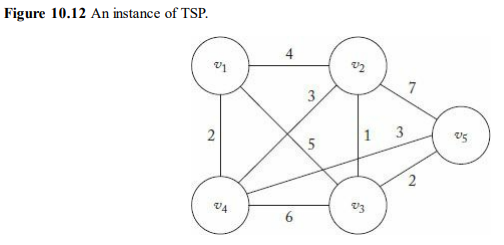
\includegraphics[width=\textwidth,keepaspectratio]{tsp.png}
    \label{fig:space_partition}
    \caption{Visualization of a KD Tree structure being used to partition points along 2 dimensional hyperplanes}
\end{figure}
There will be text after this image
\newpage
\section*{Genetic Algorithms and Financial Trading}

\end{document}